\documentclass[]{article}
\usepackage{lmodern}
\usepackage{amssymb,amsmath}
\usepackage{ifxetex,ifluatex}
\usepackage{fixltx2e} % provides \textsubscript
\ifnum 0\ifxetex 1\fi\ifluatex 1\fi=0 % if pdftex
  \usepackage[T1]{fontenc}
  \usepackage[utf8]{inputenc}
\else % if luatex or xelatex
  \ifxetex
    \usepackage{mathspec}
    \usepackage{xltxtra,xunicode}
  \else
    \usepackage{fontspec}
  \fi
  \defaultfontfeatures{Mapping=tex-text,Scale=MatchLowercase}
  \newcommand{\euro}{€}
\fi
% use upquote if available, for straight quotes in verbatim environments
\IfFileExists{upquote.sty}{\usepackage{upquote}}{}
% use microtype if available
\IfFileExists{microtype.sty}{\usepackage{microtype}}{}
\usepackage[margin=1in]{geometry}
\usepackage{graphicx}
\makeatletter
\def\maxwidth{\ifdim\Gin@nat@width>\linewidth\linewidth\else\Gin@nat@width\fi}
\def\maxheight{\ifdim\Gin@nat@height>\textheight\textheight\else\Gin@nat@height\fi}
\makeatother
% Scale images if necessary, so that they will not overflow the page
% margins by default, and it is still possible to overwrite the defaults
% using explicit options in \includegraphics[width, height, ...]{}
\setkeys{Gin}{width=\maxwidth,height=\maxheight,keepaspectratio}
\ifxetex
  \usepackage[setpagesize=false, % page size defined by xetex
              unicode=false, % unicode breaks when used with xetex
              xetex]{hyperref}
\else
  \usepackage[unicode=true]{hyperref}
\fi
\hypersetup{breaklinks=true,
            bookmarks=true,
            pdfauthor={Justin Le},
            pdftitle={Looking forward: A Doctorate Program},
            colorlinks=true,
            citecolor=blue,
            urlcolor=blue,
            linkcolor=magenta,
            pdfborder={0 0 0}}
\urlstyle{same}  % don't use monospace font for urls
% Make links footnotes instead of hotlinks:
\renewcommand{\href}[2]{#2\footnote{\url{#1}}}
\setlength{\parindent}{0pt}
\setlength{\parskip}{6pt plus 2pt minus 1pt}
\setlength{\emergencystretch}{3em}  % prevent overfull lines
\setcounter{secnumdepth}{0}

\title{Looking forward: A Doctorate Program}
\author{Justin Le}
\date{June 2, 2014}

\begin{document}
\maketitle

\emph{Originally posted on
\textbf{\href{https://blog.jle.im/entry/looking-forward-a-doctorate-program.html}{in
Code}}.}

So a bit of some personal news (which you can safely ignore if you're not
interested in my personal life!) --- I'm excited to announce that I have decided
to accept an offer to the Computational and Data Science Doctorate Program at
\href{http://www.chapman.edu/}{Chapman University} in California. I came to this
decision after a decently long period of deliberation and thinking things over,
and weighing opportunities at Chapman against my other offers. However, having
just finalized everything this week, I am ready to announce Chapman as my home
for my doctoral studies in the upcoming years.

There are two main aspects to my decision --- why computational science, and why
Chapman?

\begin{figure}
\centering
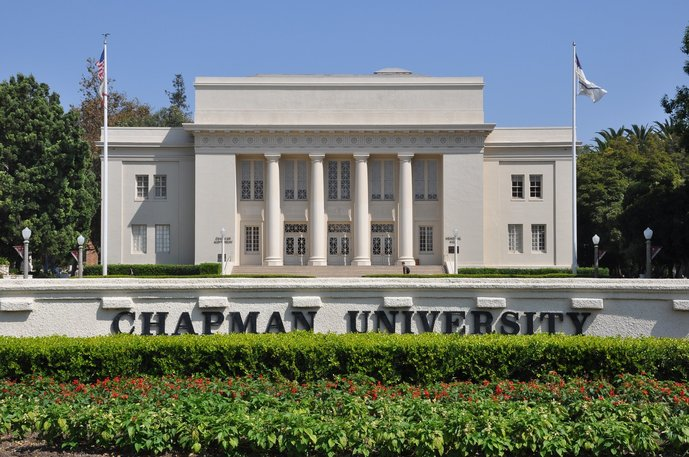
\includegraphics{/img/entries/chapman/williams-hall.jpg}
\caption{Williams Hall --- Chapman University (Photo by Tom Arthur)}
\end{figure}

\hypertarget{why-computational-science}{%
\section{Why Computational Science?}\label{why-computational-science}}

\hypertarget{from-physics}{%
\subsection{From Physics}\label{from-physics}}

For the first few years of my journey in higher education, I had always believed
that I belonged in Physics. Well, all my friends were in Physics and I didn't
really know otherwise. But even before that, there was so much I had admired
about the beauty of Physics. The quest for elegance in our models. The creation
and taming of new mathematics to fit our purposes. The relentless and ages-long
drive to unify everything into a single, beautiful framework with as few
assumptions and axioms as possible, and the fact that from such simplicity,
things weave themselves together to create such stunning complexity.

It wasn't too long before I realized that I was a little out of place amongst my
peers, and (apparently) a long tradition of physicists.

I had often remarked that I would have just as much joy in figuring out the
``physics'' of a made-up universe --- that the joy was in finding the
mathematical models that would describe it and finding out the implications.

Apparently --- and who knew! --- these days, most physicists are driven by a
desire to understand our \emph{own} physical world.

I looked back on all of the physicists of history who I admired --- Gauss,
Gibbs, Metropolis, Heisenberg --- I looked up to them for their ability to
invent and draw from new mathematics to tackle their very real problems at hand.
The fact that Gauss is just as popular in Mathematics as he is in Physics is a
true testament to his genius. And while Gibbs is known for revolutionizing
thermodynamics and statistical mechanics as we know it, I more admired the
intricate maths that he pioneered and \emph{invented}, \emph{just} to solve the
problems at hand.

Maybe, instead of taming the world, I was more fascinated with taming thought?

\hypertarget{taming-thought}{%
\subsection{Taming Thought}\label{taming-thought}}

Anyways, over the course of the first half of my final year at my undergraduate
university , I talked to more and more people and received a lot of suggestions
on what was for me. I owe a lot of where I am today to the people who helped me
during this stage, and for the people who took time out to invest in guiding me.
I found myself spending a lot of time in the Applied Maths department of my
school, and I eventually stumbled upon the field of ``Computational Science'',
which was presented to me as this interdisciplinary blend of
Physics/Engineering, Applied Mathematics, and Computer Science. It basically
involves pulling in from the entire landscape of maths and applying it to
developing new computational techniques, models, and methods in order to solve
vast and complex problems in the real world across a wide variety of domains.

Really, it seemed to represent everything that I had been interested in and was
pursuing on my own time, for the past year or two. It represented everything
that interested me in the ``real'' lab positions and jobs I took. In everything
I did, I attempted to ask ``how much of this problem can I turn into a problem
in computational science?''

The path sort of all clicked together --- in Physics, I was always a bit more
experienced in computation than my Physics peers. In Computer Science, I was
always a bit more experienced in maths than my CS peers. My peers were often
times better grounded than me in their respective fields, but I always
recognized myself as one of the few with that specific and unique
interdisciplinary blend. Surely, there were people like me --- surely I wasn't
alone. And after finding out about Computational Science, I realized that I
wasn't.

I knew that I could easily and eagerly spend my entire academic career focused
on pioneering new methods and models and theories of computation and applied
maths. And I knew that it was really what I had wanted to do all along.

Not only was it what I was apparently passionate about this entire time, I saw
it as a very important field in the coming ages. With computation and data
science more important than ever in the fields of medicine, engineering, health
care, economics, defense, artificial intelligence, and in simply rethinking the
way we live life --- I was excited to be able to be a pioneer in this new field
that had the potential to impact so many sectors of the world. It was exciting
also because it was such a new field that there was much room for innovation,
and people today still are only beginning to partially realize what was even
possible with computational science. If I can look back in sixty years at the
world around me and see a revolutionized world and believe that I had a part in
it all, I don't think I'd be regretting anything.

These were big motivations, but most of all, I was motivated in my shift by just
simply following my interests and passions. The rest is a nice bonus!

In this decision, I sort of was saying goodbye to my first love, Physics. But in
a way, I really wasn't --- this was the part of Physics that I loved this entire
time, and I am not the first in History to make this choice. I was eager to
apply all of the intuition and tools and insight that I learned from studying
Physics and finishing a B.S. on it to this field that needed --- more than any
other --- someone who came from exactly that background.

\hypertarget{why-chapman}{%
\section{Why Chapman?}\label{why-chapman}}

After doing the above soul-searching, it came time to finally send out my
applications. I collected the best of my references and wrote out my personal
statements, researched schools and faculty, and submitted my applications to a
very narrow and selective set of schools, from a variety of programs and fields
--- from Physics to Electrical Engineering to Computational Sciences (picking
from universities on this
\href{http://www.siam.org/students/resources/cse_programs.php}{useful SIAM
journal list}). I only picked programs where I felt I could apply what I
mentioned above. I was even able to manage to get a much-appreciated
recommendation from a distinguished person in the Haskell community that I
admired very much, a professor at University of California, San Diego.

The months passed and the offers and rejections came. As expected, I did not
receive an offer from my few choices in pure Physics, but I received offers from
places in Electrical Engineering and Computational Science --- Chapman among
them.

Every place I received an offer from offered their own unique benefits --- from
the reputation of a big name to strong ties in favorable industries, and the
like.

Probably the first significant event in my decision to accept Chapman's offer
was my meeting with the Chancellor, Daniele Struppa --- a brilliant
mathematician who literally embodied everything about the field that I loved. A
chancellor who still was active in research, he showed me how he himself worked
in the fields of biology, geology, meteorology, and ontology, and many more by
simply looking at the problems and linking concepts of applied mathematics. With
knowledge of the wider context of applied maths, he was able to look into
problems and find just the tool that was missing.

He shared with me his vision of Chapman's future in the sciences, and much of it
reflected his own philosophy. He dreamed of expanding Chapman as an established
name into industries and fields I was excited to be a part of. And I saw myself
able to not only be a part of a growing field but to also be a part of a new
movement and a very grand vision of an up-and-coming science university, and
maybe (just maybe!) even being able to help shape it.

The fact that Chapman was home to an impressive list of top world physicists
(including a 2013 Nobel Laureate involved in discovering the Higgs mechanism)
didn't hurt either!

Still, even with this, I still was not yet fully decided. My other offers were
from schools that weren't just up-and-coming --- they were already established!

However, when I looked at their doctorate programs (in comparison to Chapman's),
I couldn't help but feel like I'd be compromising myself. Other departments had
aspects that I could apply what I was passionate about to. They had advisors an
teams that I could --- if I twisted myself in just the right way --- apply my
interests towards. However, everything about Chapman's program seemed to just
fit like a glove. The objective, the courses, and the projects and advisers, as
I began to realize, were almost as if they were lifted straight from my dream
school --- my dream program! If I could write my own doctoral program,
environment, and culture, it would almost exactly match the environment,
culture, and program of Chapman.

When I realized that, I realized that I had made my decision.

\hypertarget{onward}{%
\section{Onward}\label{onward}}

So\ldots that's it. I'll probably be using this coming summer to transition into
Chapman and the faculty there, and maybe find a team I could try to contribute
to. And then I'll be starting in the fall. I'm excited to see how this journey
winds up in four years, but I know that this is the start of an exciting next
stage of my life!

\hypertarget{signoff}{%
\section{Signoff}\label{signoff}}

Hi, thanks for reading! You can reach me via email at
\href{mailto:justin@jle.im}{\nolinkurl{justin@jle.im}}, or at twitter at
\href{https://twitter.com/mstk}{@mstk}! This post and all others are published
under the \href{https://creativecommons.org/licenses/by-nc-nd/3.0/}{CC-BY-NC-ND
3.0} license. Corrections and edits via pull request are welcome and encouraged
at \href{https://github.com/mstksg/inCode}{the source repository}.

If you feel inclined, or this post was particularly helpful for you, why not
consider \href{https://www.patreon.com/justinle/overview}{supporting me on
Patreon}, or a \href{bitcoin:3D7rmAYgbDnp4gp4rf22THsGt74fNucPDU}{BTC donation}?
:)

\end{document}
